% Created 2023-09-09 sáb 11:37
% Intended LaTeX compiler: pdflatex
\documentclass[aspectratio=169, 9pt]{beamer}
\usepackage[utf8]{inputenc}
\usepackage[T1]{fontenc}
\usepackage{graphicx}
\usepackage{grffile}
\usepackage{longtable}
\usepackage{wrapfig}
\usepackage{rotating}
\usepackage[normalem]{ulem}
\usepackage{amsmath}
\usepackage{textcomp}
\usepackage{amssymb}
\usepackage{capt-of}
\usepackage{hyperref}
\usepackage{../modernpres}
\bibliography{../sample.bib}
\usetheme{default}
\setcounter{secnumdepth}{2}
\author{Luis Eduardo Galindo Amaya (1274895) \\
Juan Fransisco Perez Valdez  (324342)}
\date{29 de Junio 2023}
\title{Identificación y manejo de \\
material de laboratorio}
\hypersetup{
 pdfauthor={Luis Eduardo Galindo Amaya (1274895) \\
Juan Fransisco Perez Valdez  (324342)},
 pdftitle={Identificación y manejo de \\
material de laboratorio},
 pdfkeywords={},
 pdfsubject={},
 pdfcreator={Emacs 27.1 (Org mode 9.3)}, 
 pdflang={Spanish}}
\begin{document}

\maketitle

\begin{frame}[label={sec:org99c4775}]{Hola como estas}
\begin{figure}[htbp]
\centering
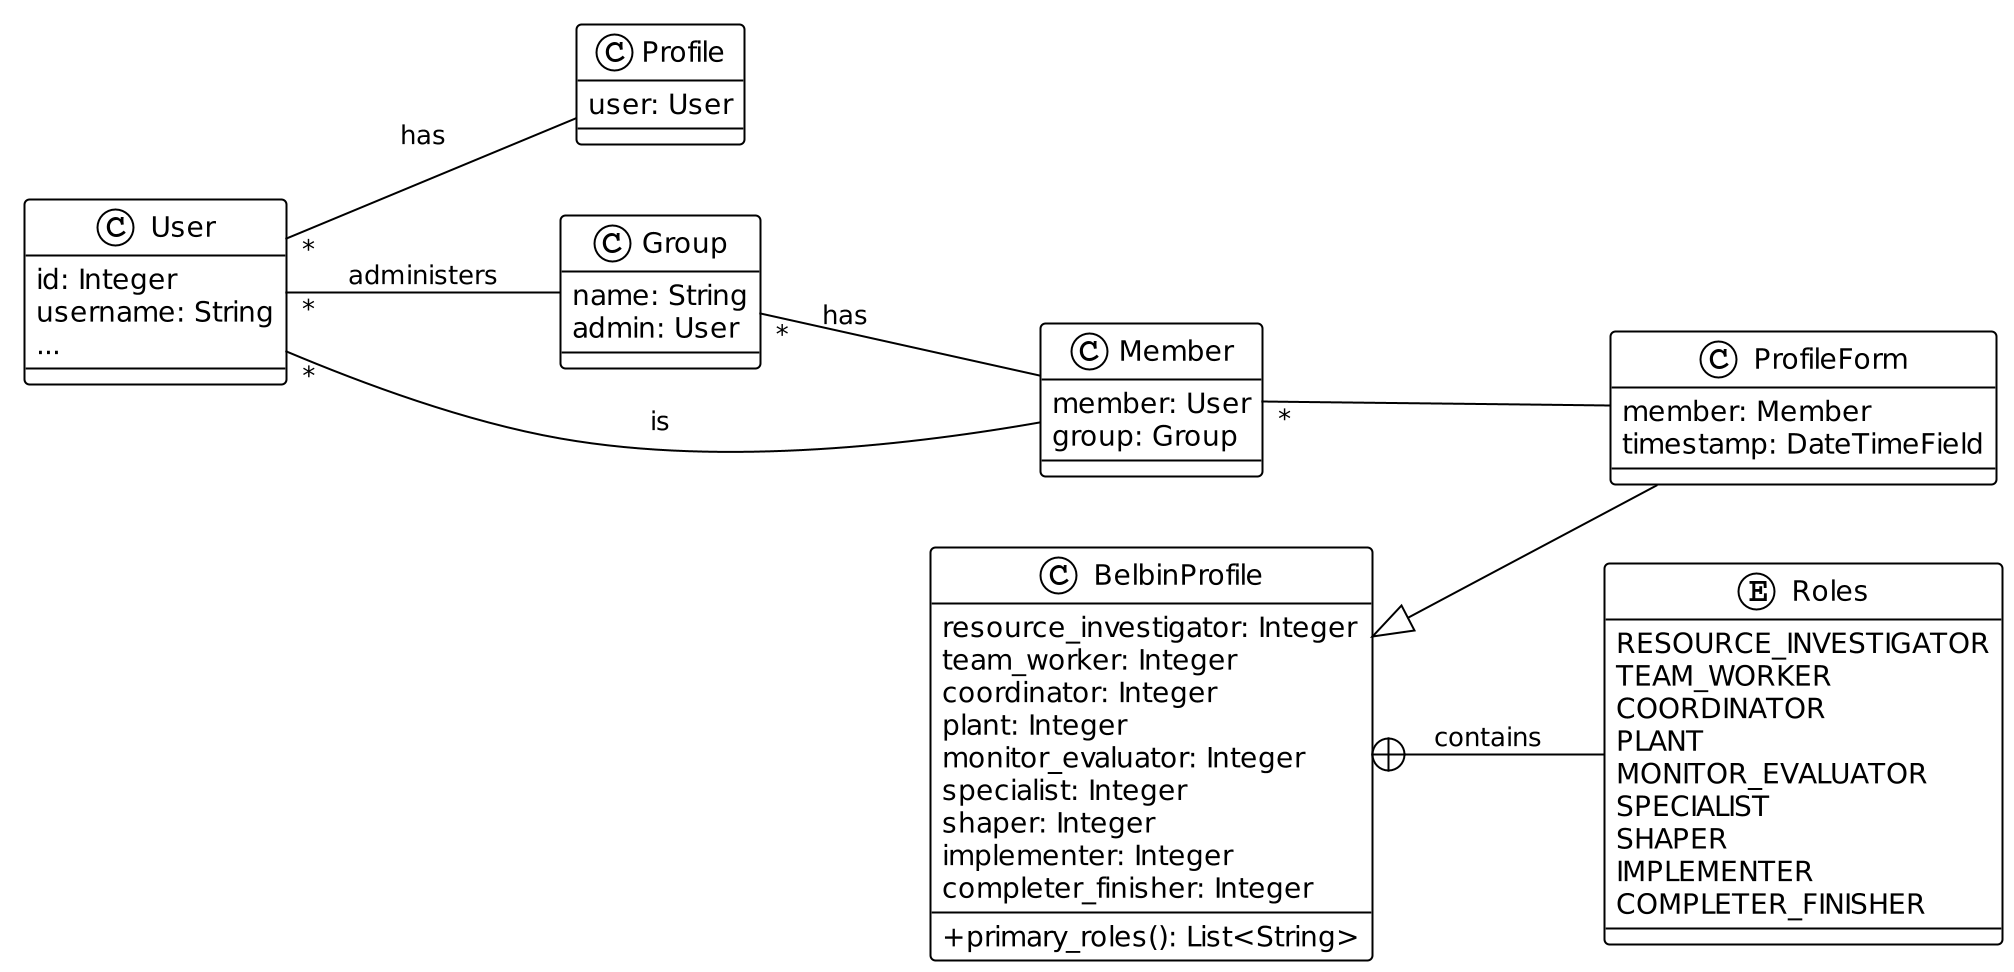
\includegraphics[width=.9\linewidth]{./images/dmulti.png}
\caption{hola como estan en este dia de la vida (\cite{einstein}).}
\end{figure}
\end{frame}

\begin{frame}[label={sec:orgbce1b32}]{Pie de pagina y listas}
\begin{block}{Hola como estan}
Pellentesque dapibus suscipit ligula.  Donec posuere augue in quam.  Etiam vel
tortor sodales tellus ultricies commodo.  Suspendisse potenti.  Aenean in sem 
ac leo mollis blandit.  Donec neque quam, dignissim in, mollis \footnote{\cite{russell}}
nec, sagittis eu \footnote{Etiam vel tortor sodales tellus ultricies commodo}. 

\begin{itemize}
\item Como estan
\begin{enumerate}
\item en este dia
\item de la lvida
\end{enumerate}
\end{itemize}
\end{block}
\end{frame}

\begin{frame}[label={sec:orgf4366d8},fragile]{Código}
 \begin{verbatim}
import Yesod

data WebApp = WebApp Yesod WebApp

mkYesod "WebApp" [parseRoutes|
  / HomeR GET
|]

getHomeR = defaultLayout [whamlet|
  <div>Hello, world!
|]

main = warpEnv WebApp

mkYesod "WebApp" [parseRoutes|
  / HomeR GET
|]

yay
veinte parece el limite
\end{verbatim}
\captionof{figure}{Esta es una prueba}
\end{frame}

\begin{frame}[label={sec:org490eb83}]{Tablas}
\[ \iint x^2 + y^2 - 1 \,dx \,dy \]
\begin{center}
\begin{tabular}{|l|l|}
Test 1 & Test 2\\
Hola & esta es una pruba\\
\end{tabular}

\end{center}
\end{frame}

\begin{frame}[label={sec:org1f1fd42}]{Media pagina vertical}
Proin quam nisl, tincidunt et, mattis eget, convallis nec, purus\footnote{Hola este es un test de footnote}.
In id erat non orci commodo lobortis.  Phasellus purus. 

\begin{figure}[htbp]
\centering
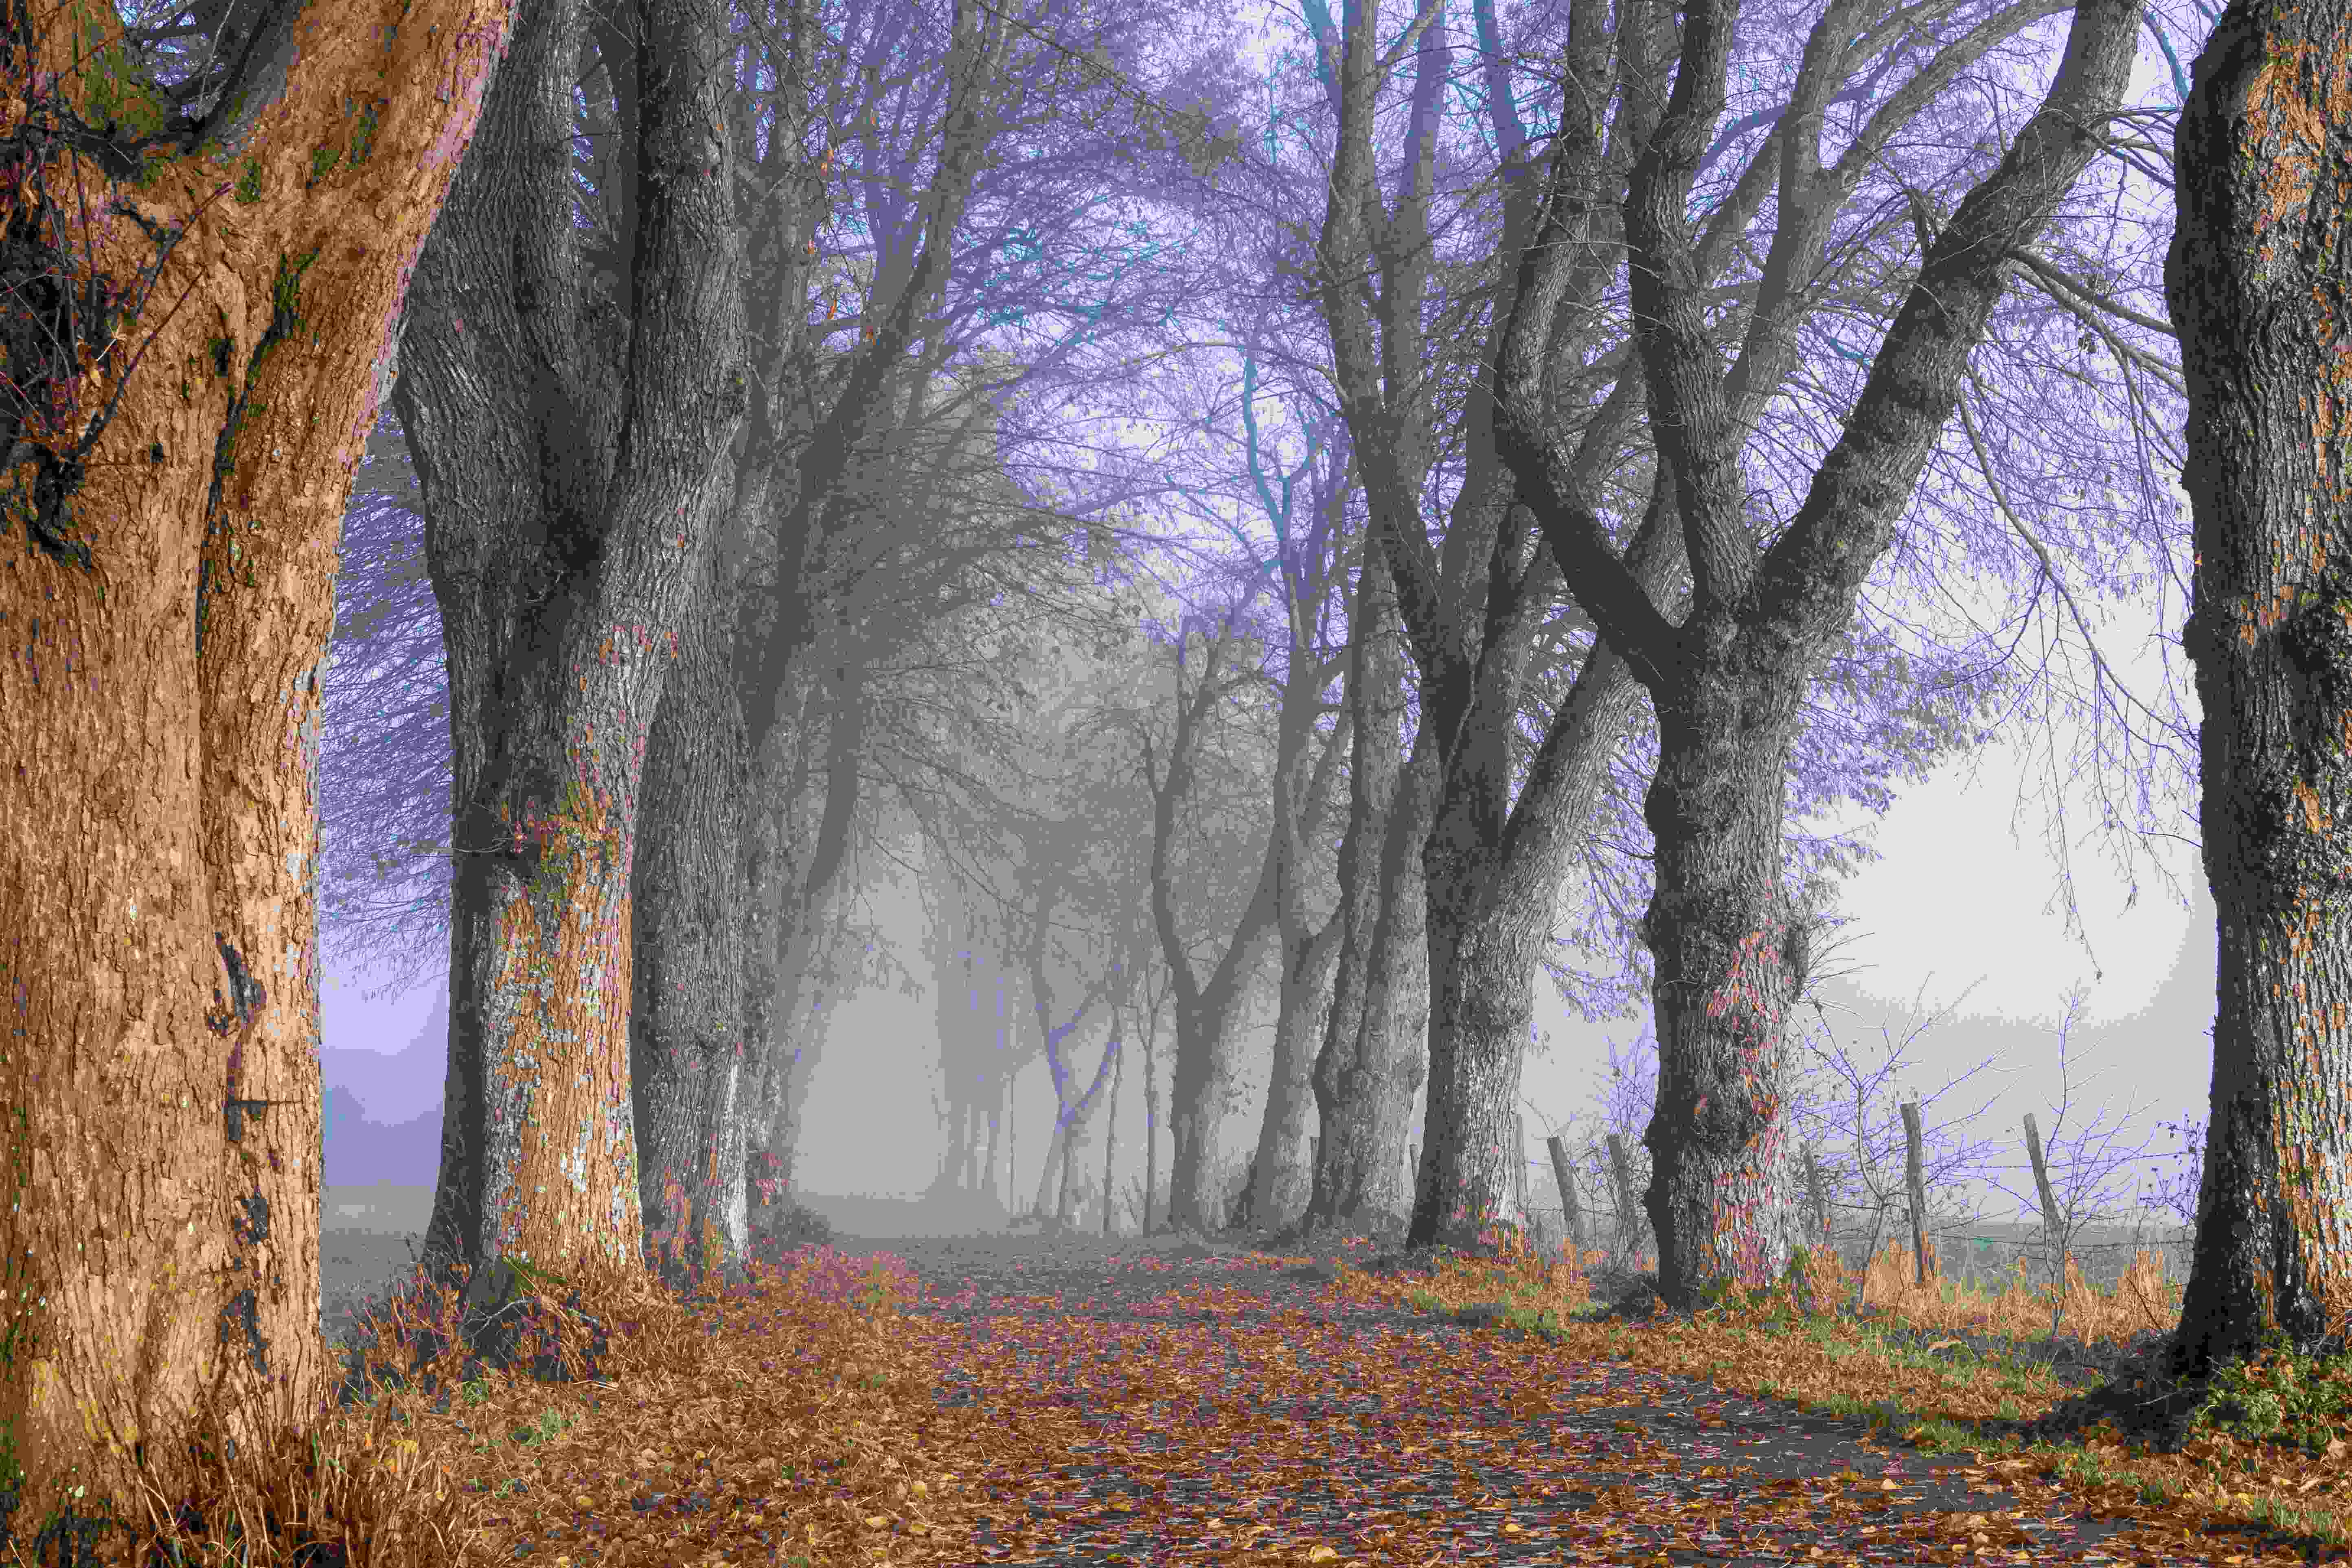
\includegraphics[width=200px]{images/2019-11-30-Marienallee_Dahlem-7978.jpg}
\caption{Este es un test de una imagen}
\end{figure}
\end{frame}

\begin{frame}[label={sec:org9be4e44}]{Media pagina horizontal}
\begin{twoc}
\alert{Hack de subtitulos} \\
The plot with teal color corresponds to the function \(y=(x^3-1)^2\) and the plot
with red color corresponds to the function \(y=(x^{11}-1)^2\)   
\end{twoc}
\begin{threec}
\begin{figure}[htbp]
\centering
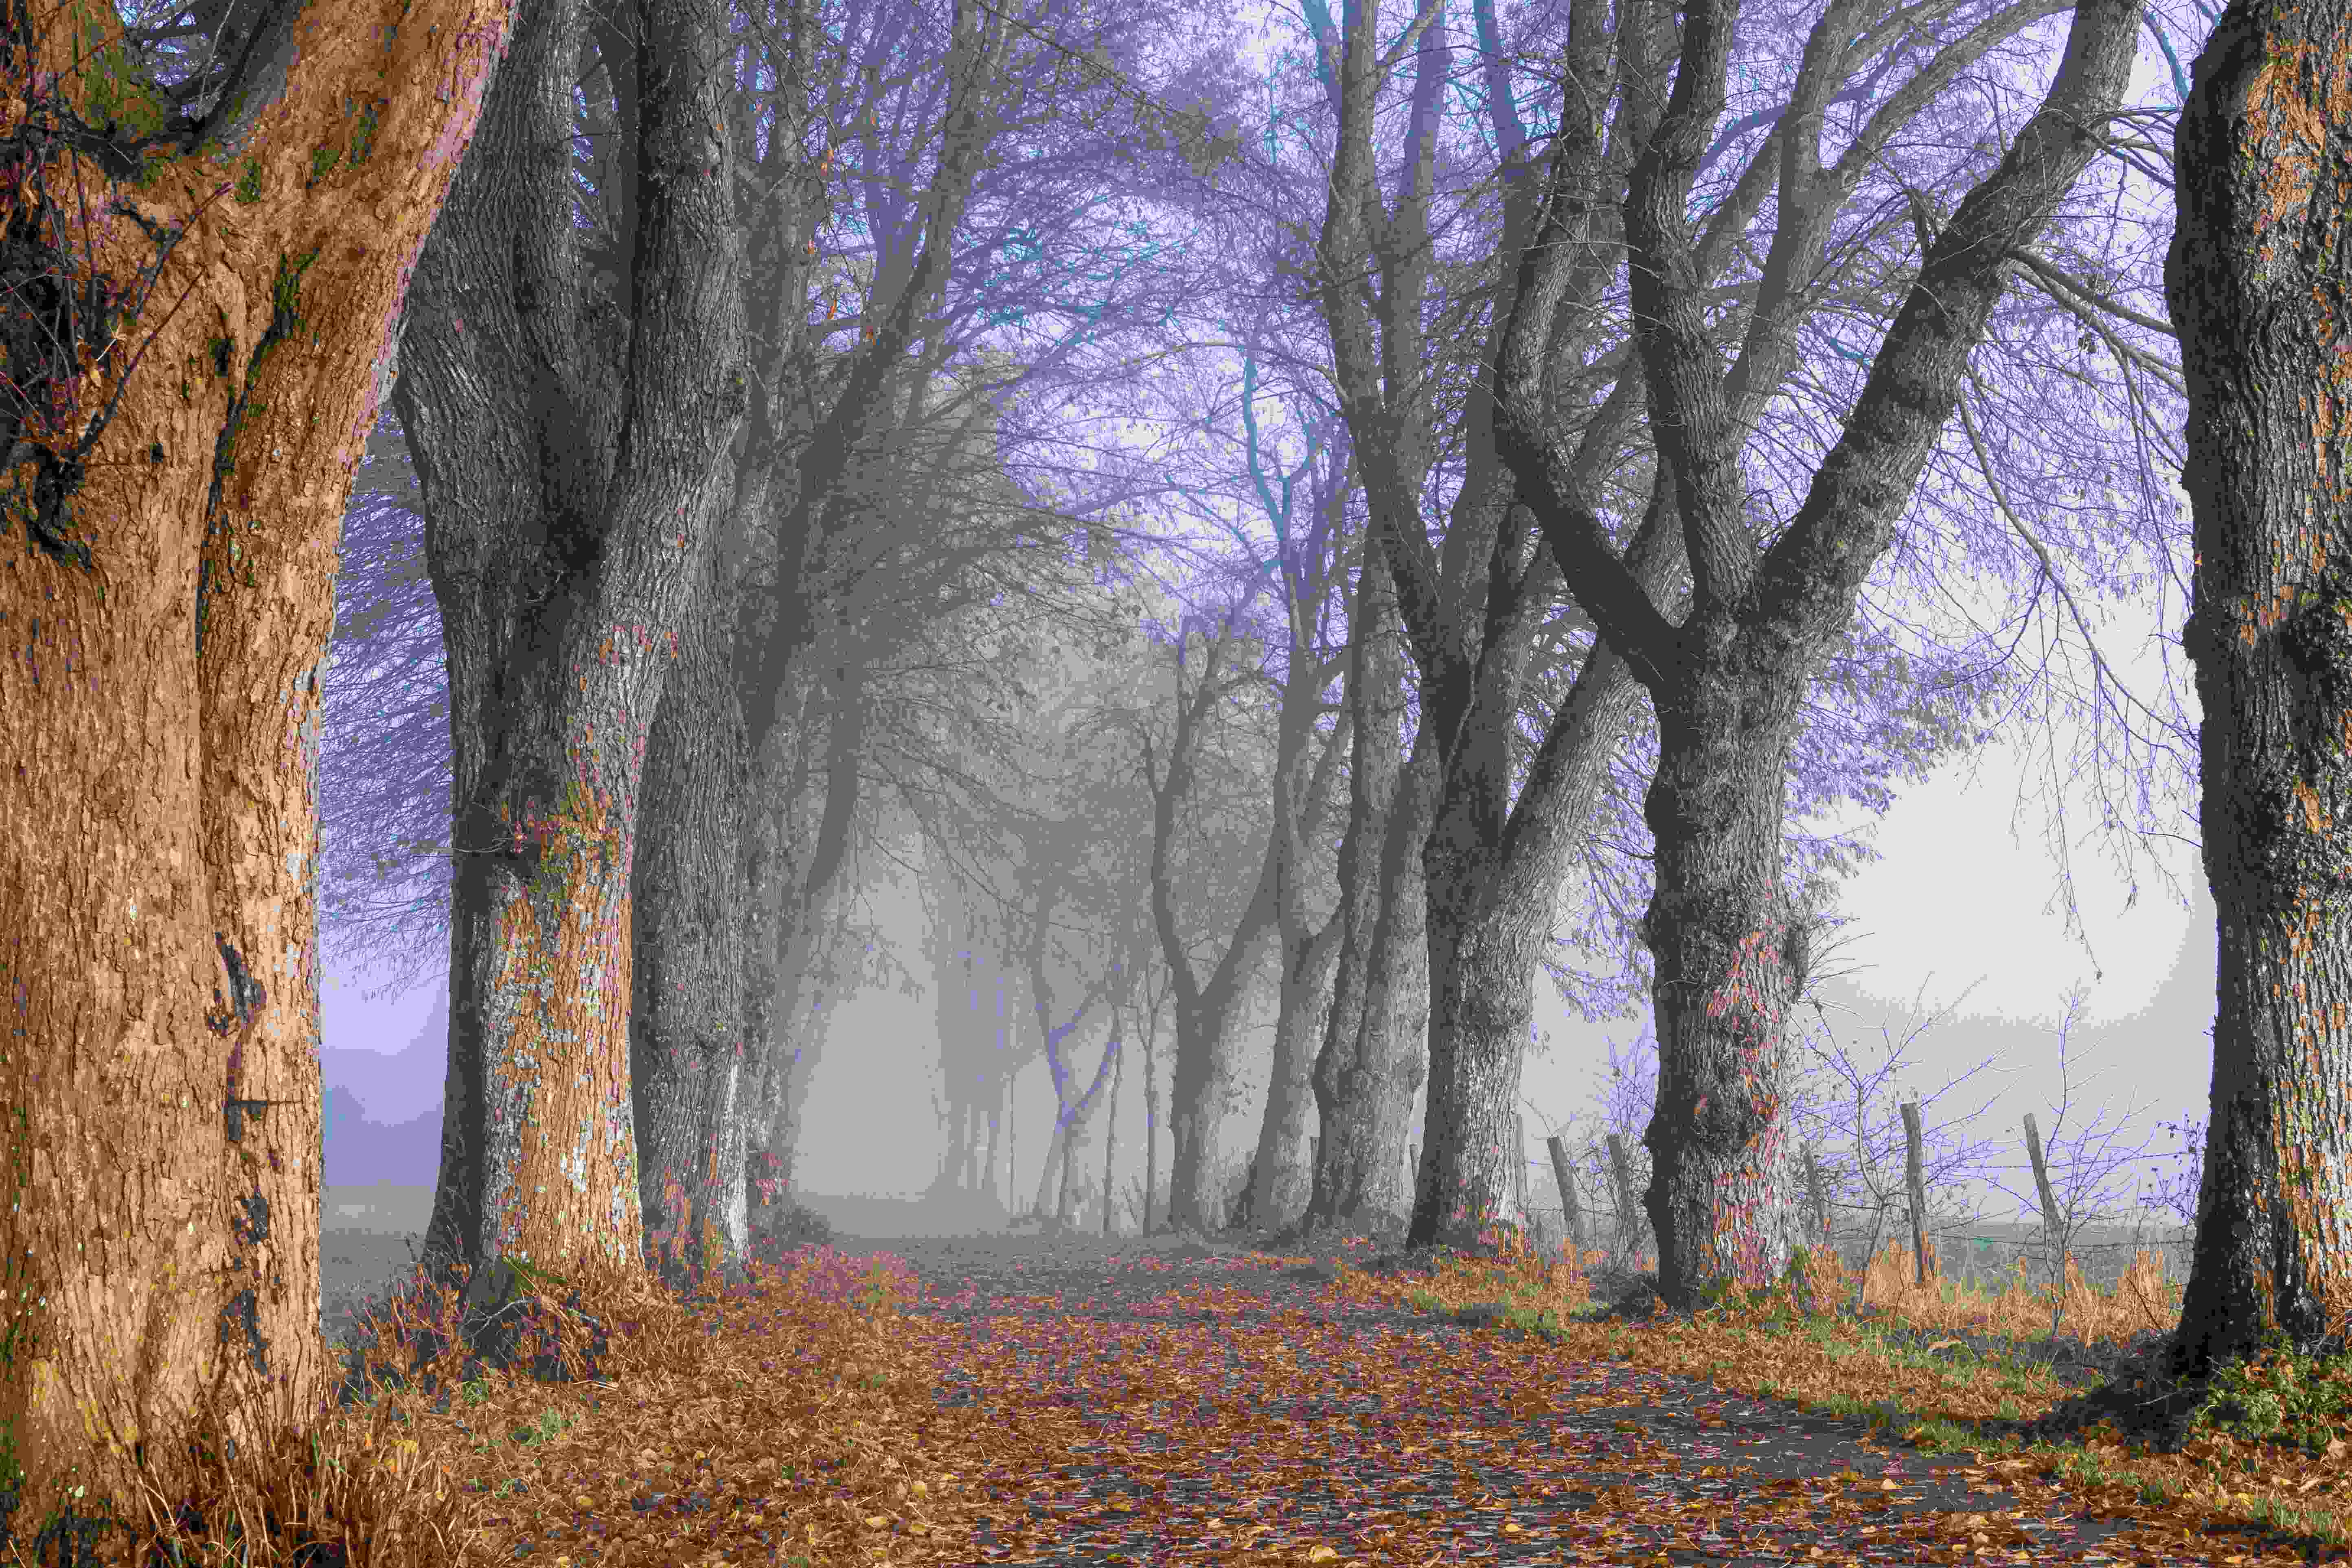
\includegraphics[width=.9\linewidth]{images/2019-11-30-Marienallee_Dahlem-7978.jpg}
\caption{hola como estan}
\end{figure}
\end{threec}
\end{frame}

\begin{frame}[label={sec:orgbe3b247},fragile]{Código mediapagina}
 \begin{threec}
\begin{verbatim}
import Yesod

data WebApp = WebApp Yesod WebApp

mkYesod "WebApp" [parseRoutes|
  / HomeR GET
|]

getHomeR = defaultLayout [whamlet|
  <div>Hello, world!
|]

main = warpEnv WebApp

mkYesod "WebApp" [parseRoutes|
  / HomeR GET
|]

yay
veinte parece el limite
dfsfd
fdsfsd
fdsfds
fdsfd
\end{verbatim}
\end{threec}
\begin{twoc}
\alert{Otro Hack} \\
The plot with teal color corresponds to the function \(y=(x^3-1)^2\) and the plot
with red color corresponds to the function \(y=(x^{11}-1)^2\)
\end{twoc}
\end{frame}

\begin{frame}[label={sec:orgc0672f0}]{Test de sección}
\begin{quote}
Aliquam erat volutpat.  Nunc eleifend leo vitae magna.  In id erat non orci
commodo lobortis.  Proin neque massa, cursus ut, gravida ut, lobortis eget, 
lacus.  Sed diam.  Praesent fermentum tempor tellus.  Nullam tempus.  Mauris 
erat.
\end{quote}

\begin{alertblock}{Conclusio    n}
Simmons Hall $\not=$ Simmons Dormitory.
\end{alertblock}
\end{frame}

\begin{frame}[label={sec:org88f2167}]{Referencias}
\printbibliography
\end{frame}
\end{document}
